% Options for packages loaded elsewhere
\PassOptionsToPackage{unicode}{hyperref}
\PassOptionsToPackage{hyphens}{url}
%
\documentclass[
  8pt,
  ignorenonframetext,
]{beamer}
\usepackage{pgfpages}
\setbeamertemplate{caption}[numbered]
\setbeamertemplate{caption label separator}{: }
\setbeamercolor{caption name}{fg=normal text.fg}
\beamertemplatenavigationsymbolsempty
% Prevent slide breaks in the middle of a paragraph
\widowpenalties 1 10000
\raggedbottom
\setbeamertemplate{part page}{
  \centering
  \begin{beamercolorbox}[sep=16pt,center]{part title}
    \usebeamerfont{part title}\insertpart\par
  \end{beamercolorbox}
}
\setbeamertemplate{section page}{
  \centering
  \begin{beamercolorbox}[sep=12pt,center]{part title}
    \usebeamerfont{section title}\insertsection\par
  \end{beamercolorbox}
}
\setbeamertemplate{subsection page}{
  \centering
  \begin{beamercolorbox}[sep=8pt,center]{part title}
    \usebeamerfont{subsection title}\insertsubsection\par
  \end{beamercolorbox}
}
\AtBeginPart{
  \frame{\partpage}
}
\AtBeginSection{
  \ifbibliography
  \else
    \frame{\sectionpage}
  \fi
}
\AtBeginSubsection{
  \frame{\subsectionpage}
}
\usepackage{amsmath,amssymb}
\usepackage{lmodern}
\usepackage{iftex}
\ifPDFTeX
  \usepackage[T1]{fontenc}
  \usepackage[utf8]{inputenc}
  \usepackage{textcomp} % provide euro and other symbols
\else % if luatex or xetex
  \usepackage{unicode-math}
  \defaultfontfeatures{Scale=MatchLowercase}
  \defaultfontfeatures[\rmfamily]{Ligatures=TeX,Scale=1}
\fi
% Use upquote if available, for straight quotes in verbatim environments
\IfFileExists{upquote.sty}{\usepackage{upquote}}{}
\IfFileExists{microtype.sty}{% use microtype if available
  \usepackage[]{microtype}
  \UseMicrotypeSet[protrusion]{basicmath} % disable protrusion for tt fonts
}{}
\makeatletter
\@ifundefined{KOMAClassName}{% if non-KOMA class
  \IfFileExists{parskip.sty}{%
    \usepackage{parskip}
  }{% else
    \setlength{\parindent}{0pt}
    \setlength{\parskip}{6pt plus 2pt minus 1pt}}
}{% if KOMA class
  \KOMAoptions{parskip=half}}
\makeatother
\usepackage{xcolor}
\newif\ifbibliography
\usepackage{color}
\usepackage{fancyvrb}
\newcommand{\VerbBar}{|}
\newcommand{\VERB}{\Verb[commandchars=\\\{\}]}
\DefineVerbatimEnvironment{Highlighting}{Verbatim}{commandchars=\\\{\}}
% Add ',fontsize=\small' for more characters per line
\usepackage{framed}
\definecolor{shadecolor}{RGB}{248,248,248}
\newenvironment{Shaded}{\begin{snugshade}}{\end{snugshade}}
\newcommand{\AlertTok}[1]{\textcolor[rgb]{0.94,0.16,0.16}{#1}}
\newcommand{\AnnotationTok}[1]{\textcolor[rgb]{0.56,0.35,0.01}{\textbf{\textit{#1}}}}
\newcommand{\AttributeTok}[1]{\textcolor[rgb]{0.77,0.63,0.00}{#1}}
\newcommand{\BaseNTok}[1]{\textcolor[rgb]{0.00,0.00,0.81}{#1}}
\newcommand{\BuiltInTok}[1]{#1}
\newcommand{\CharTok}[1]{\textcolor[rgb]{0.31,0.60,0.02}{#1}}
\newcommand{\CommentTok}[1]{\textcolor[rgb]{0.56,0.35,0.01}{\textit{#1}}}
\newcommand{\CommentVarTok}[1]{\textcolor[rgb]{0.56,0.35,0.01}{\textbf{\textit{#1}}}}
\newcommand{\ConstantTok}[1]{\textcolor[rgb]{0.00,0.00,0.00}{#1}}
\newcommand{\ControlFlowTok}[1]{\textcolor[rgb]{0.13,0.29,0.53}{\textbf{#1}}}
\newcommand{\DataTypeTok}[1]{\textcolor[rgb]{0.13,0.29,0.53}{#1}}
\newcommand{\DecValTok}[1]{\textcolor[rgb]{0.00,0.00,0.81}{#1}}
\newcommand{\DocumentationTok}[1]{\textcolor[rgb]{0.56,0.35,0.01}{\textbf{\textit{#1}}}}
\newcommand{\ErrorTok}[1]{\textcolor[rgb]{0.64,0.00,0.00}{\textbf{#1}}}
\newcommand{\ExtensionTok}[1]{#1}
\newcommand{\FloatTok}[1]{\textcolor[rgb]{0.00,0.00,0.81}{#1}}
\newcommand{\FunctionTok}[1]{\textcolor[rgb]{0.00,0.00,0.00}{#1}}
\newcommand{\ImportTok}[1]{#1}
\newcommand{\InformationTok}[1]{\textcolor[rgb]{0.56,0.35,0.01}{\textbf{\textit{#1}}}}
\newcommand{\KeywordTok}[1]{\textcolor[rgb]{0.13,0.29,0.53}{\textbf{#1}}}
\newcommand{\NormalTok}[1]{#1}
\newcommand{\OperatorTok}[1]{\textcolor[rgb]{0.81,0.36,0.00}{\textbf{#1}}}
\newcommand{\OtherTok}[1]{\textcolor[rgb]{0.56,0.35,0.01}{#1}}
\newcommand{\PreprocessorTok}[1]{\textcolor[rgb]{0.56,0.35,0.01}{\textit{#1}}}
\newcommand{\RegionMarkerTok}[1]{#1}
\newcommand{\SpecialCharTok}[1]{\textcolor[rgb]{0.00,0.00,0.00}{#1}}
\newcommand{\SpecialStringTok}[1]{\textcolor[rgb]{0.31,0.60,0.02}{#1}}
\newcommand{\StringTok}[1]{\textcolor[rgb]{0.31,0.60,0.02}{#1}}
\newcommand{\VariableTok}[1]{\textcolor[rgb]{0.00,0.00,0.00}{#1}}
\newcommand{\VerbatimStringTok}[1]{\textcolor[rgb]{0.31,0.60,0.02}{#1}}
\newcommand{\WarningTok}[1]{\textcolor[rgb]{0.56,0.35,0.01}{\textbf{\textit{#1}}}}
\usepackage{longtable,booktabs,array}
\usepackage{calc} % for calculating minipage widths
\usepackage{caption}
% Make caption package work with longtable
\makeatletter
\def\fnum@table{\tablename~\thetable}
\makeatother
\setlength{\emergencystretch}{3em} % prevent overfull lines
\providecommand{\tightlist}{%
  \setlength{\itemsep}{0pt}\setlength{\parskip}{0pt}}
\setcounter{secnumdepth}{-\maxdimen} % remove section numbering
% type setting
% ------------------------------------------------------------------------------
\usepackage[german]{babel}     

% fonts
% ------------------------------------------------------------------------------
\usefonttheme{professionalfonts}

% slide title and horizontal line
% ------------------------------------------------------------------------------
\setbeamertemplate{frametitle}{%
    \vskip-30pt \color{black}\large%
    \begin{minipage}[b][23pt]{120mm}%
    \flushleft\insertframetitle%
    \end{minipage}%
}

\setbeamertemplate{headline}										
{
\vskip10pt\hfill\hspace{3.5mm} 										 
\vskip15pt\color{black}\rule{\textwidth}{0.4pt} 					 
}

% slide number
% ---------------------------------------------------------------
\setbeamertemplate{navigation symbols}{}
\setbeamertemplate{footline}
{
\vskip5pt
\vskip2pt
\makebox[123mm]{\hspace{7.5mm}
\hfill Wahrscheinlichkeitstheorie und Frequentistische Inferenz $\vert$ 
\copyright $ $ 2023 Dirk Ostwald CC BY-SA 4.0 $\vert$ 
Folie \insertframenumber}
\vskip4pt
}

% block color scheme
% ------------------------------------------------------------------------------
% colors
\definecolor{white}{RGB}{255,255,255}
\definecolor{grey}{RGB}{235,235,235}
\definecolor{lightgrey}{RGB}{245,245,245}
\definecolor{LightBlue}{RGB}{220,220,255}
\definecolor{darkblue}{RGB}{51, 51, 153}

% definitions and theorems
\setbeamercolor{block title}{fg = black, bg = grey}
\setbeamercolor{block body}{fg = black, bg = lightgrey}

% general line spacing 
% ------------------------------------------------------------------------------
\linespread{1.3}

% local line spacing
% ------------------------------------------------------------------------------
\usepackage{setspace}

% colors
% -----------------------------------------------------------------------------
\usepackage{color}

% justified text
% ------------------------------------------------------------------------------
\usepackage{ragged2e}
\usepackage{etoolbox}
\apptocmd{\frame}{}{\justifying}{}

% bullet point lists
% -----------------------------------------------------------------------------
\setbeamertemplate{itemize item}[circle]
\setbeamertemplate{itemize subitem}[circle]
\setbeamertemplate{itemize subsubitem}[circle]
\setbeamercolor{itemize item}{fg = black}
\setbeamercolor{itemize subitem}{fg = black}
\setbeamercolor{itemize subsubitem}{fg = black}
\setbeamercolor{enumerate item}{fg = black}
\setbeamercolor{enumerate subitem}{fg = black}
\setbeamercolor{enumerate subsubitem}{fg = black}
\setbeamerfont{itemize/enumerate body}{}
\setbeamerfont{itemize/enumerate subbody}{size = \normalsize}
\setbeamerfont{itemize/enumerate subsubbody}{size = \normalsize}

% color links
% ------------------------------------------------------------------------------
\usepackage{hyperref}
\definecolor{urls}{RGB}{204,0,0}
\hypersetup{colorlinks, citecolor = darkblue, urlcolor = urls}


% additional math commands
% ------------------------------------------------------------------------------
\usepackage{bm}                                         
\newcommand{\niton}{\not\owns}
\newcommand{\ups}{\upsilon}


% text highlighting
% ------------------------------------------------------------------------------
\usepackage{soul}
\makeatletter
\let\HL\hl
\renewcommand\hl{%
  \let\set@color\beamerorig@set@color
  \let\reset@color\beamerorig@reset@color
  \HL}
\makeatother

% equation highlighting
% -----------------------------------------------------------------------------
\newcommand{\highlight}[2][yellow]{\mathchoice%
  {\colorbox{#1}{$\displaystyle#2$}}%
  {\colorbox{#1}{$\textstyle#2$}}%
  {\colorbox{#1}{$\scriptstyle#2$}}%
  {\colorbox{#1}{$\scriptscriptstyle#2$}}}%

% additional mathematical operators
% ------------------------------------------------------------------------------
\DeclareMathOperator*{\argmax}{arg\,max}
\DeclareMathOperator*{\argmin}{arg\,min}
\DeclareMathOperator*{\intinf}{\int_{-\infty}^{\infty}}
\ifLuaTeX
  \usepackage{selnolig}  % disable illegal ligatures
\fi
\IfFileExists{bookmark.sty}{\usepackage{bookmark}}{\usepackage{hyperref}}
\IfFileExists{xurl.sty}{\usepackage{xurl}}{} % add URL line breaks if available
\urlstyle{same} % disable monospaced font for URLs
\hypersetup{
  hidelinks,
  pdfcreator={LaTeX via pandoc}}

\author{}
\date{\vspace{-2.5em}}

\begin{document}

\begin{frame}[plain]{}
\protect\hypertarget{section}{}
\center

\begin{center}
\includegraphics[width=0.2\linewidth]{9_Abbildungen/wtfi_9_otto} \end{center}

\vspace{2mm}

\Large

Wahrscheinlichkeitstheorie und Frequentistische Inferenz \vspace{6mm}

\large

BSc Psychologie WiSe 2022/23

\vspace{6mm}
\normalsize

Prof.~Dr.~Dirk Ostwald
\end{frame}

\begin{frame}[plain]{}
\protect\hypertarget{section-1}{}
\vfill
\center
\huge

\textcolor{black}{(9) Grundbegriffe Frequentistischer Inferenz} \vfill
\end{frame}

\begin{frame}{}
\protect\hypertarget{section-2}{}
\center
\footnotesize
\renewcommand{\arraystretch}{1.1}
\begin{tabular}{lll}
Datum        & Einheit                       & Thema                                                \\\hline
13.10.2022   & Einführung                    & (1) Einführung                                       \\
20.10.2022   & Wahrscheinlichkeitstheorie    & (2) Wahrscheinlichkeitsräume                         \\
27.10.2022   & Wahrscheinlichkeitstheorie    & (3) Elementare Wahrscheinlichkeiten                  \\
03.11.2022   & Wahrscheinlichkeitstheorie    & (4) Zufallsvariablen I                               \\
10.11.2022   & Wahrscheinlichkeitstheorie    & (4) Zufallsvariablen II                              \\
17.11.2022   & Wahrscheinlichkeitstheorie    & (5) Multivariate Verteilungen                        \\
24.11.2022   & Wahrscheinlichkeitstheorie    & (6) Erwartungswert und Kovarianz                     \\
01.12.2022   & Wahrscheinlichkeitstheorie    & (7) Ungleichungen und Grenzwerte                     \\
08.12.2022   & Wahrscheinlichkeitstheorie    & (8) Transformationen der Normalverteilung            \\
15.12.2022   & Frequentistische Inferenz     & (9) Grundbegriffe Frequentistischer Inferenz         \\
             & \textcolor{gray}{Weihnachtspause}                                                    \\
05.01.2023   & Frequentistische Inferenz     & (10) Parameterschätzung                              \\
12.01.2023   & Frequentistische Inferenz     & (11) Konfidenzintervalle                             \\
19.01.2023   & Frequentistische Inferenz     & (12) Hypothesentests I                               \\
26.01.2023   & Frequentistische Inferenz     & (12) Hypothesentests II                              \\\hline
02.02.2023   & Klausur                       & G44-H6, 16:00 - 17:00 Uhr                            \\
Jul 2023     & Klausurwiederholungstermin    &
\end{tabular}
\end{frame}

\begin{frame}{}
\protect\hypertarget{section-3}{}
\textcolor{darkblue}{Modellbasierte Datenwissenschaft} \vspace{3mm}

\begin{center}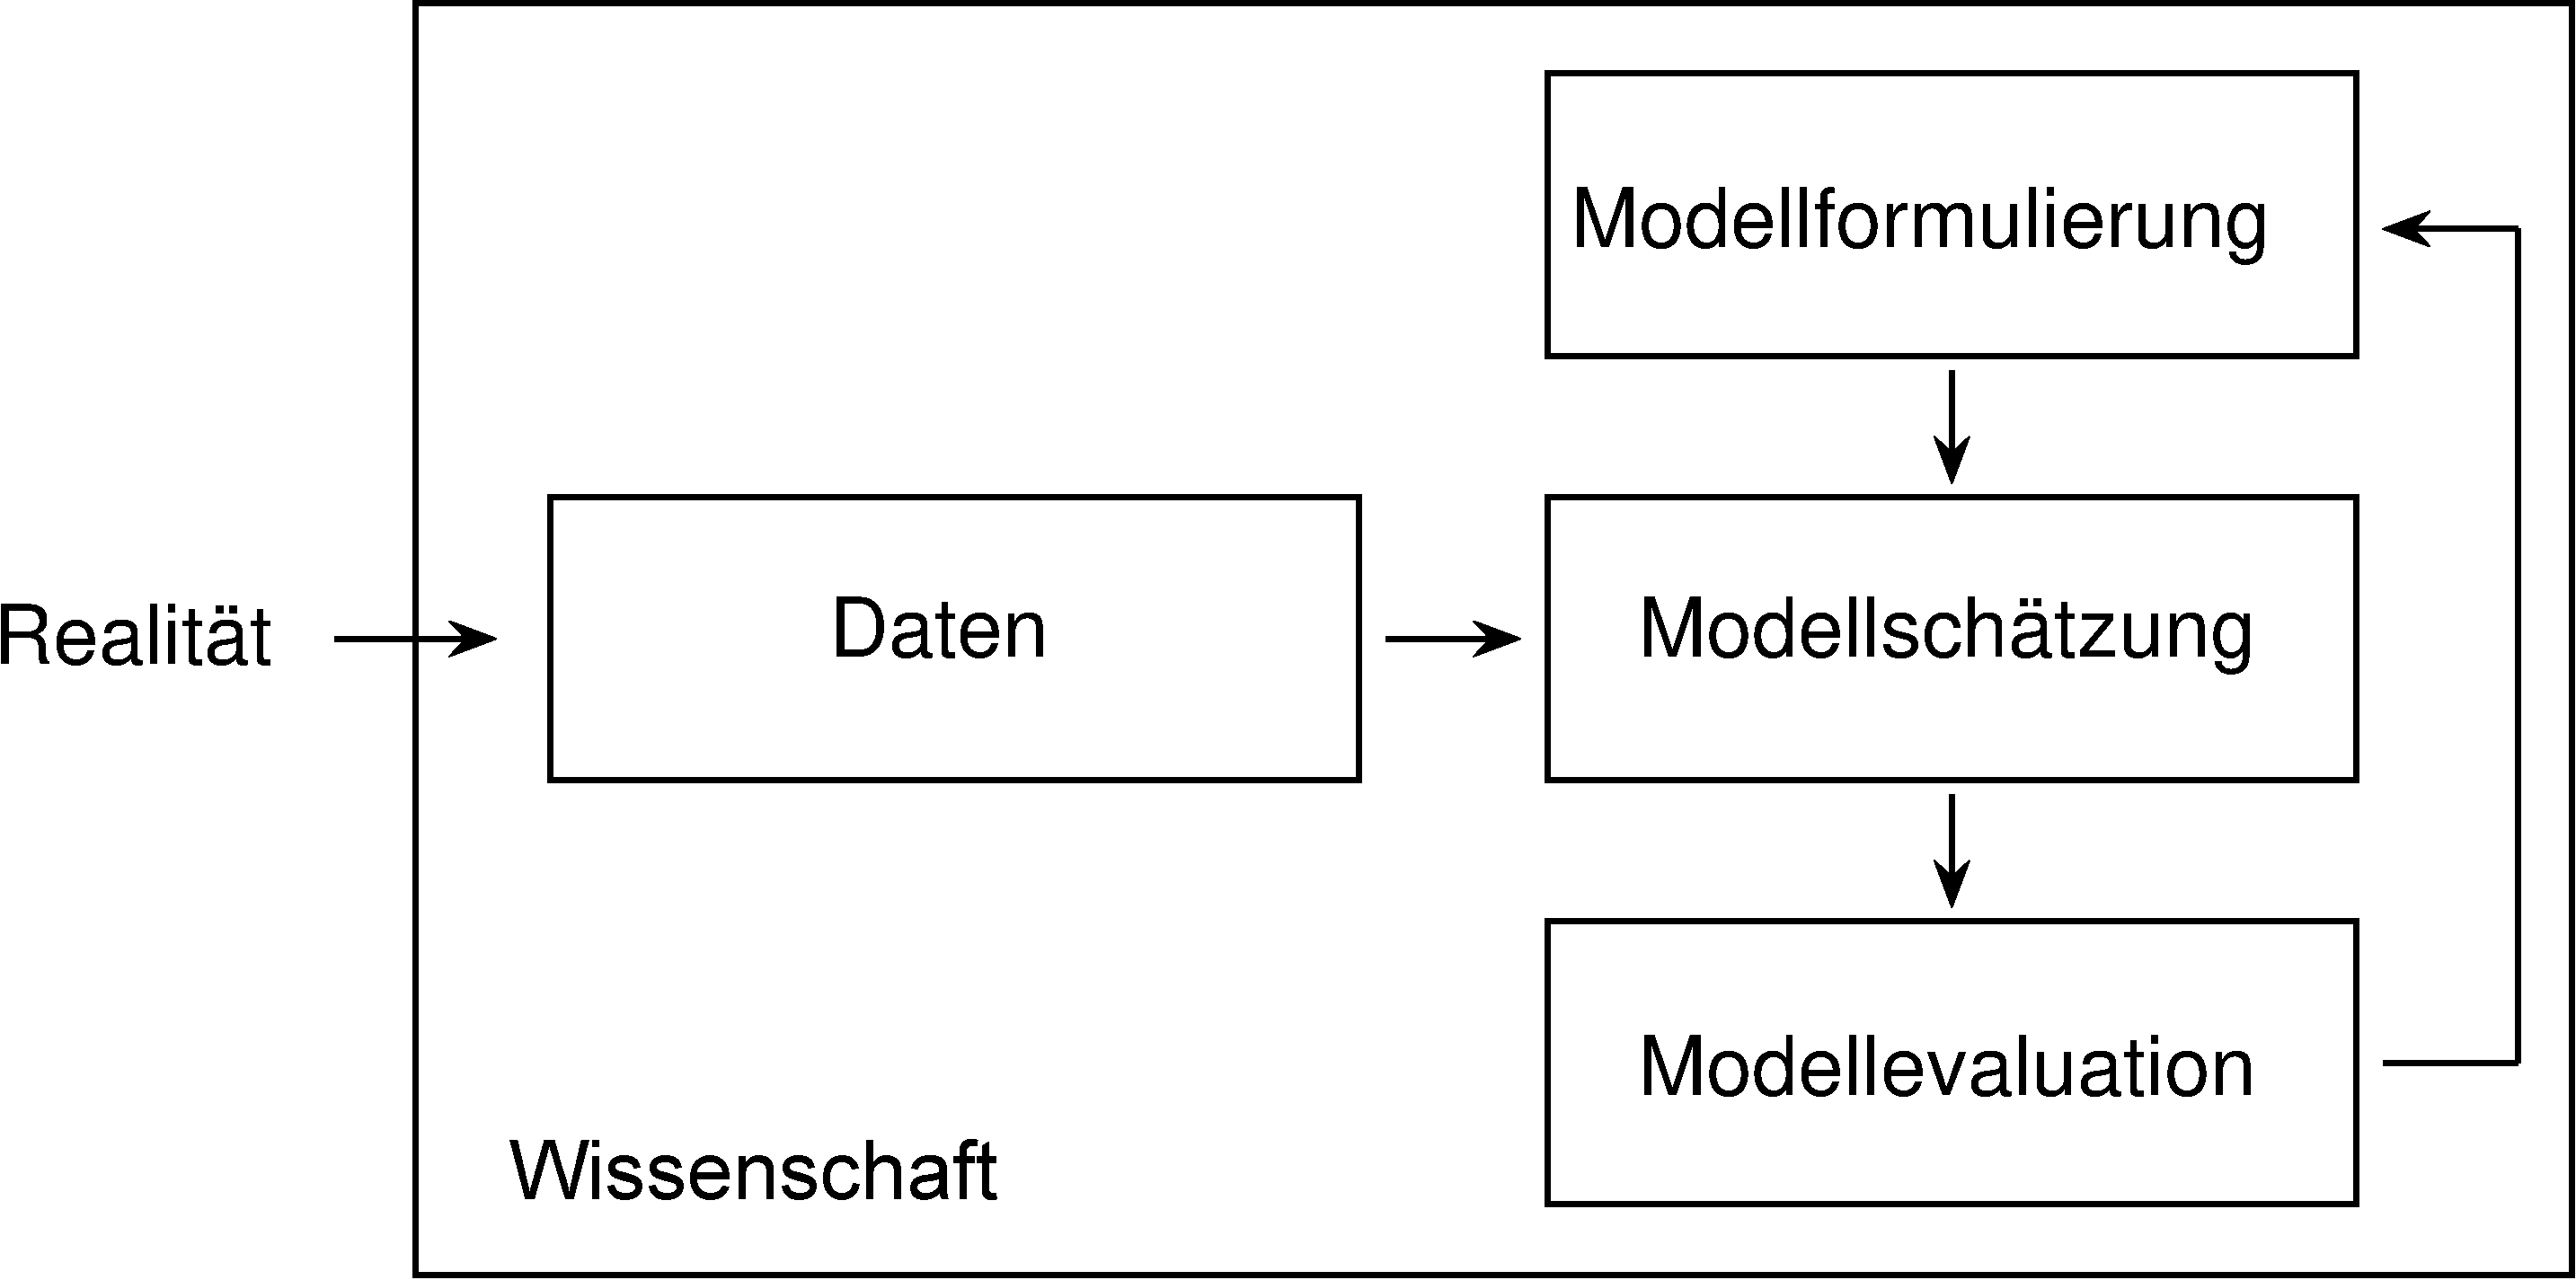
\includegraphics[width=0.75\linewidth]{9_Abbildungen/wtfi_9_modellbasierte_datenwissenschaft} \end{center}

\textcolor{darkblue}{Frequentistische Inferenz} \small \vspace{3mm}
\center

\begin{tabular}{ll}
Modellformulierung & $\Rightarrow$ Statistische Modelle                                \\
Modellschätzung    & $\Rightarrow$ Parameterschätzung und Konfidenzintervalle          \\
Modellevaluation   & $\Rightarrow$ Hypothesentests (cf. Allgemeines Lineares Modell)
\end{tabular}
\end{frame}

\begin{frame}{}
\protect\hypertarget{section-4}{}
\large
\setstretch{3}
\vfill

Statistische Modelle

Statistiken und Schätzer

Standardprobleme Frequentistischer Inferenz

Selbstkontrollfragen \vfill
\end{frame}

\begin{frame}{}
\protect\hypertarget{section-5}{}
\large
\setstretch{3}
\vfill

\textbf{Statistische Modelle}

Statistiken und Schätzer

Standardprobleme Frequentistischer Inferenz

Selbstkontrollfragen \vfill
\end{frame}

\begin{frame}{Statistische Modelle}
\protect\hypertarget{statistische-modelle}{}
\footnotesize
\begin{definition}[Statistisches Modell]
\justifying
Ein \textit{statistisches Modell} ist ein Tripel
\begin{equation}
\mathcal{M} := (\mathcal{Y}, \mathcal{A}, \{\mathbb{P}_\theta |\theta \in \Theta\})
\end{equation}
bestehend  aus einem \textit{Datenraum} $\mathcal{Y}$, einer $\sigma$-Algebra
$\mathcal{A}$ auf $\mathcal{Y}$ und einer mindestens zweielementigen Menge
$\{\mathbb{P}_\theta |\theta \in \Theta\}$ von Wahrscheinlichkeitsmaßen auf
$(\mathcal{Y}, \mathcal{A})$, die durch $\theta \in \Theta$ indiziert sind.
Wenn $\Theta \subset \mathbb{R}^k$ ist, heißt ein statistisches Modell auch \textit{parametrisches} 
statistisches Modell und $\Theta$ heißt \textit{Parameterraum} des statistischen Modells.
\end{definition}

\footnotesize

Bemerkungen

\begin{itemize}
\tightlist
\item
  Für Erwartungswerte und (Ko)Varianzen bezüglich \(\mathbb{P}_\theta\)
  schreiben wir \(\mathbb{E}_\theta\), \(\mathbb{V}_\theta\),
  \(\mathbb{C}_\theta\).
\item
  \justifying Ein statistisches Modell \(\mathcal{M}\) heißt ein
  \emph{diskretes Modell}, wenn \(\mathcal{Y}\) diskret ist und jedes
  \(\mathbb{P}_\theta\) eine WMF \(p_\theta\) besitzt,\\
  ein statistisches Modell \(\mathcal{M}\) heißt ein \emph{stetiges
  Modell}, wenn \(\mathcal{Y} \subset \mathbb{R}^n\) ist und jedes
  \(\mathbb{P}_\theta\) eine WDF \(p_\theta\) besitzt.
\item
  Für ein statistisches Modell
  \(\mathcal{M}_0 := (\mathcal{Y}_0, \mathcal{A}_0, \{\mathbb{P}_\theta^0 |\theta \in \Theta\})\)
  heißt das statistische Modell
  \(\mathcal{M} := (\mathcal{Y}, \mathcal{A}, \{\mathbb{P}_\theta |\theta \in \Theta\})\),
  für das \(\mathcal{Y}\) das \(n\)-fache kartesische Produkt von
  \(\mathcal{Y}_0\) mit sich selbst, \(\mathcal{A}\) die entsprechende
  Produkt-\(\sigma\)-Algebra ist, und
  \(\{\mathbb{P}_\theta |\theta \in \Theta\}\) die entsprechende Menge
  an Produktmaßen ist, das zu \(\mathcal{M}_0\) gehörige
  \emph{Produktmodell}.
\item
  Wenn für ein Produktmodell die Menge \(\mathcal{Y}_0\) eindimensional
  ist, also z.B. \(\mathcal{Y}_0 = \mathbb{R}\) gilt, spricht man von
  einem \emph{univariaten statistischen Modell}. Wenn für ein
  Produktmodell die Menge \(\mathcal{Y}_0\) mehrdimensional ist, also
  z.B. \(\mathcal{Y}_0 = \mathbb{R}^m, m > 1\) ist, spricht man von
  einem \emph{multivariaten statistischen Modell}.
\end{itemize}
\end{frame}

\begin{frame}{Statistische Modelle}
\protect\hypertarget{statistische-modelle-1}{}
\footnotesize

Bemerkungen (fortgeführt)

\begin{itemize}
\item
  \justifying Der Vorgang der Datenbeobachtung wird durch einen
  Zufallsvektor \(\ups\), der Werte in \(\mathcal{Y}\) annimmt,
  beschrieben. Im Kontext statistischer Modelle nennt man diesen
  Zufallsvektor \emph{Daten}, \emph{Beobachtung}, \emph{Messung} oder
  \emph{Stichprobe}. Eine Realisierung von \(\ups\), also konkret
  vorliegende Datenwerte \(y \in \mathcal{Y}\), werden \emph{Datensatz},
  \emph{Beobachtungswert}, \emph{Messwert} oder \emph{Stichprobenwert}
  genannt.
\item
  \justifying Produktmodelle modellieren die \(n\)-fache unabhängige
  Wiederholung eines Zufallsvorgangs. Der entsprechende Zufallsvektor
  \(\ups := (\ups_1,....,\ups_n)\) entspricht dann einer Menge von \(n\)
  unabhängigen Zufallsvariablen.
\item
  \justifying Im Gegensatz zum Wahrscheinlichkeitsraummodell betrachtet
  man bei statistische Modellen zwei oder mehr Wahrscheinlichkeitsmaße,
  die die Verteilung von \(\ups\) mutmaßlich bestimmen. Das jeweils
  zugrundeliegende Wahrscheinlichkeitsmaß ist mit \(\theta \in \Theta\)
  indiziert,
\item
  \justifying In einem konkreten Datenanalyseproblem nimmt man an, dass
  die beobachteten Werte \(y = (y_1,...,y_n)\) von
  \(\ups = (\ups_1,...,\ups_n)\) durch \(\theta^*\) generiert wurde,
  wobei \(\theta^*\) hier den \emph{wahren, aber unbekannten,
  Parameterwert} bezeichnet. Der wahre, aber unbekannten, Parameterwert
  \(\theta^*\) bleibt auch nach der statistischen Analyse unbekannt. In
  der mathematischen Analyse von Inferenzmethoden betrachtet man alle
  möglichen wahren, aber unbekannten, Parameterwerte, schreibt also
  einfach \(\{\mathbb{P}_\theta |\theta \in \Theta\}\).
\end{itemize}
\end{frame}

\begin{frame}{Statistische Modelle}
\protect\hypertarget{statistische-modelle-2}{}
\footnotesize
\begin{definition}[Normalverteilungsmodell]
Das univariate parametrische Produktmodell
\begin{equation}
\mathcal{M} := \left(\mathcal{Y}, \mathcal{A}, \{\mathbb{P}_\theta|\theta \in \Theta\}\right)
\end{equation}
mit
\begin{equation}
\mathcal{Y} := \mathbb{R}^n, \mathcal{A} := \mathcal{B}(\mathbb{R}^n), \theta := (\mu, \sigma^2), \Theta := \mathbb{R} \times \mathbb{R}_{>0},
\end{equation}
also
\begin{equation}
\{\mathbb{P}_\theta|\theta \in \Theta\}
:= \left\lbrace \prod_{i=1}^n N(\mu,\sigma^2)|(\mu,\sigma^2)\in \mathbb{R} \times \mathbb{R}_{>0} \right\rbrace,
\end{equation}
und damit
\begin{equation}
\ups_1,...,\ups_n \sim N(\mu,\sigma^2) \mbox{ mit } (\mu,\sigma^2)\in \mathbb{R} \times \mathbb{R}_{>0}
\end{equation}
heißt \textit{Normalverteilungsmodell}.
\end{definition}
\footnotesize

Bemerkungen

\begin{itemize}
\tightlist
\item
  \justifying Das Normalverteilungsmodell ist Grundlage vieler populärer
  statistischen Verfahren.
\item
  Diese Verfahren werden im Allgemeinen Linearen Modell integrativ
  betrachtet.
\item
  Das Modell ist grundlegend durch normalverteilte Fehlerterme
  motiviert.
\end{itemize}
\end{frame}

\begin{frame}{Statistische Modelle}
\protect\hypertarget{statistische-modelle-3}{}
\footnotesize
\begin{definition}[Bernoullimodell]
Das univariate parametrische Produktmodell
\begin{equation}
\mathcal{M} := \left(\mathcal{Y}, \mathcal{A}, \{\mathbb{P}_\theta|\theta \in \Theta\}\right)
\end{equation}
mit
\begin{equation}
\mathcal{Y} := \{0,1\}^n, \mathcal{A} := \mathcal{P}\left(\{0,1\}^n\right), \theta:= \mu, \Theta := ]0,1[,
\end{equation}
also
\begin{equation}
\{\mathbb{P}_\theta|\theta \in \Theta\} := \left\lbrace \prod_{i=1}^n \mbox{Bern}(\mu)|\mu \in ]0,1[ \right\rbrace,
\end{equation}
und damit
\begin{equation}
\ups_1,...,\ups_n \sim \mbox{Bern}(\mu) \mbox{ mit } \mu \in ]0,1[,
\end{equation}
heißt \textit{Bernoullimodell}.
\end{definition}

\footnotesize

Bemerkung

\begin{itemize}
\tightlist
\item
  Das Bernoullimodell spielt in der statistischen Anwendung eine eher
  untegeordnete Rolle.
\end{itemize}
\end{frame}

\begin{frame}{}
\protect\hypertarget{section-6}{}
\large
\setstretch{3}
\vfill

Statistische Modelle

\textbf{Statistiken und Schätzer}

Standardprobleme Frequentistischer Inferenz

Selbstkontrollfragen \vfill
\end{frame}

\begin{frame}{Statistiken und Schätzer}
\protect\hypertarget{statistiken-und-schuxe4tzer}{}
\small
\begin{definition}[Statistik]
\justifying
$\mathcal{M}$ sei ein statistisches Modell und $(\Sigma,\mathcal{S})$ sei ein Messraum.
Dann wird eine Zufallsvariable der Form
\begin{equation}
S : \mathcal{Y} \to \Sigma
\end{equation}
\textit{Statistik} genannt.
\end{definition}

Bemerkungen

\begin{itemize}
\tightlist
\item
  \justifying Daten und Statistiken werden durch Zufallsvariablen
  modelliert. Statistiken modellieren dabei von
  Datenwissenschaftler:innen konstruierte Funktionen, die bestenfalls
  datenbasierte Information liefern, aus der sich Schlüsse über die
  latenten datengenerierenden Prozesse ziehen lassen.
\end{itemize}
\end{frame}

\begin{frame}{Statistiken und Schätzer}
\protect\hypertarget{statistiken-und-schuxe4tzer-1}{}
\small

Beispiele (Statistiken)

\small

\(\mathcal{M}\) sei das Normalverteilungsmodell. Dann sind zum Beispiel
folgende Zufallsvariablen Statistiken, was wir hier explizit durch die
Notation deutlich machen wollen, was aber oft zur Vereinfachung der
Notation implizit (aber trotzdem wichtig) bleibt:

\begin{itemize}
\tightlist
\item
  Das \textit{Stichprobenmittel} \begin{equation}
  \bar{y}_n : \mathbb{R}^n \to \mathbb{R},
  y \mapsto \bar{y}_n(y) := \frac{1}{n}\sum_{i=1}^n y_i,
  \end{equation}
\item
  Die \textit{Stichprobenvarianz} \begin{equation}
  s^2_n  : \mathbb{R}^n \to \mathbb{R}_{\ge 0},
  y \mapsto s^2_n(y) := \frac{1}{n-1}\sum_{i=1}^n (y_i - \bar{y}_n(y))^2,
  \end{equation}
\item
  Die \textit{Stichprobenstandardabweichung} \begin{equation}
  s_n  : \mathbb{R}^n \to \mathbb{R}_{\ge 0},
  y \mapsto s_n(y) := \sqrt{s_n^2(y)},
  \end{equation}
\end{itemize}
\end{frame}

\begin{frame}{Statistiken und Schätzer}
\protect\hypertarget{statistiken-und-schuxe4tzer-2}{}
\small
\begin{definition}[Schätzer]
\justifying
$\mathcal{M}$ sei ein statistisches Modell, $(\Sigma,\mathcal{S})$ sei ein Messraum  
und $\tau : \Theta \to \Sigma$ sei eine Abbildung, die jedem $\theta \in \Theta$ 
eine Kenngröße $\tau(\theta) \in \Sigma$ zuordnet. Dann heißt eine Statistik 
\begin{equation}
\hat{\tau} : \mathcal{Y} \to \Sigma
\end{equation}
ein \textit{Schätzer} für $\tau$.
\end{definition}

\small

Bemerkungen

\begin{itemize}
\tightlist
\item
  Typische Beispiele für \(\tau\) sind

  \begin{itemize}
  \begin{small}
  \item[$\circ$] $\tau(\theta) := \theta$ für die Schätzung von $\theta$,
  \item[$\circ$] $\tau(\theta) := \theta_i$ mit $\theta \in \mathbb{R}^d, d > 1$ für die Schätzung einer Komponente von $\theta$,
  \item[$\circ$] $\tau(\theta) := \mathbb{E}_\theta(y_1)$ für die Schätzung des Erwartungswert,
  \item[$\circ$] $\tau(\theta) := \mathbb{V}_\theta(y_1)$ für die Schätzung der Varianz.
  \end{small}
  \end{itemize}
\item
  Für \(\hat{\tau}\) bei \(\tau(\theta) := \theta\) schreibt man
  üblicherweise \(\hat{\theta}\).
\item
  Schätzer nehmen Zahlwerte in \(\Sigma\) an und heißen deshalb auch
  \emph{Punktschätzer}.
\item
  Nicht jeder Schätzer ist ein guter Schätzer, man definiert deshalb
  \emph{Schätzgütekriterien}.
\item
  Gütekriterien für Schätzer sind der Inhalt von Vorlesungseinheit (10)
  Parameterschätzung.
\end{itemize}
\end{frame}

\begin{frame}{Statistiken und Schätzer}
\protect\hypertarget{statistiken-und-schuxe4tzer-3}{}
\small

Beispiele (Schätzer)

\(\mathcal{M}\) sei das Normalverteilungsmodell.

\begin{itemize}
\tightlist
\item
  Dann ist zum Beispiel das Stichprobenmittel
  \(\bar{y}_n : \mathbb{R}^n \to \mathbb{R}\) ein Schätzer für
  \begin{equation}
  \tau : \mathbb{R} \times \mathbb{R}_{>0} \to \mathbb{R},
  (\mu, \sigma^2) \mapsto \tau(\mu,\sigma^2) := \mu.
  \end{equation} Ebenso ist \(\bar{y}_n\) ein Schätzer für
  \begin{equation}
  \tau: \mathbb{R} \times \mathbb{R}_{>0} \to \mathbb{R},
  (\mu, \sigma_2) \mapsto \tau(\mu,\sigma^2) := \mathbb{E}_{\mu,\sigma^2}(y_1).
  \end{equation}
\item
  Weiterhin ist die konstante Funktion \begin{equation}
  \hat{\tau} : \mathbb{R}^n \to \mathbb{R}, y \mapsto \hat{\tau}(y) := 42
  \end{equation} ein Schätzer für \begin{equation}
  \tau : \mathbb{R} \times \mathbb{R}_{>0} \to \mathbb{R}_{>0},
  (\mu, \sigma_2) \mapsto \tau(\mu,\sigma^2) := \sigma^2.
  \end{equation}
\end{itemize}

Dass eine Funktion \(\hat{\tau} : \mathcal{Y} \to \Sigma\) ein Schätzer
ist, heißt nicht, dass sie ein guter Schätzer ist!
\end{frame}

\begin{frame}{}
\protect\hypertarget{section-7}{}
\large
\setstretch{3}
\vfill

Statistische Modelle

Statistiken und Schätzer

\textbf{Standardprobleme Frequentistischer Inferenz}

Selbstkontrollfragen \vfill
\end{frame}

\begin{frame}{Standardprobleme Frequentistischer Inferenz}
\protect\hypertarget{standardprobleme-frequentistischer-inferenz}{}
\small

Mithilfe statistischer Modelle behandelt die Frequentistische Inferenz
folgende Standardprobleme:

\vspace{2mm}

\noindent (1) Parameterschätzung

Ziel der Parameterschätzung ist es, einen möglichst guten Tipp für
wahre, aber unbekannte, Parameterwerte oder Funktionen dieser abzugeben,
typischerweise mithilfe der Daten.

\vspace{2mm}

\noindent (2) Konfidenzintervalle

Ziel der Bestimmung von Konfidenzintervallen ist es, basierend auf der
angenommenen Verteilung der Daten eine quantitative Aussage über die mit
Schätzwerten assoziierte Unsicherheit zu treffen.

\vspace{2mm}

\noindent (3) Hypothesentests

Ziel des Hypothesentestens ist es, basierend auf der angenommenen
Verteilung der Daten in einer möglichst zuverlässigen Form zu
entscheiden, ob ein wahrer, aber unbekannter Parameterwert in einer von
zwei sich gegenseitig ausschließenden Untermengen des Parameterraumes
liegt.
\end{frame}

\begin{frame}{Standardprobleme Frequentistischer Inferenz}
\protect\hypertarget{standardprobleme-frequentistischer-inferenz-1}{}
\begin{center}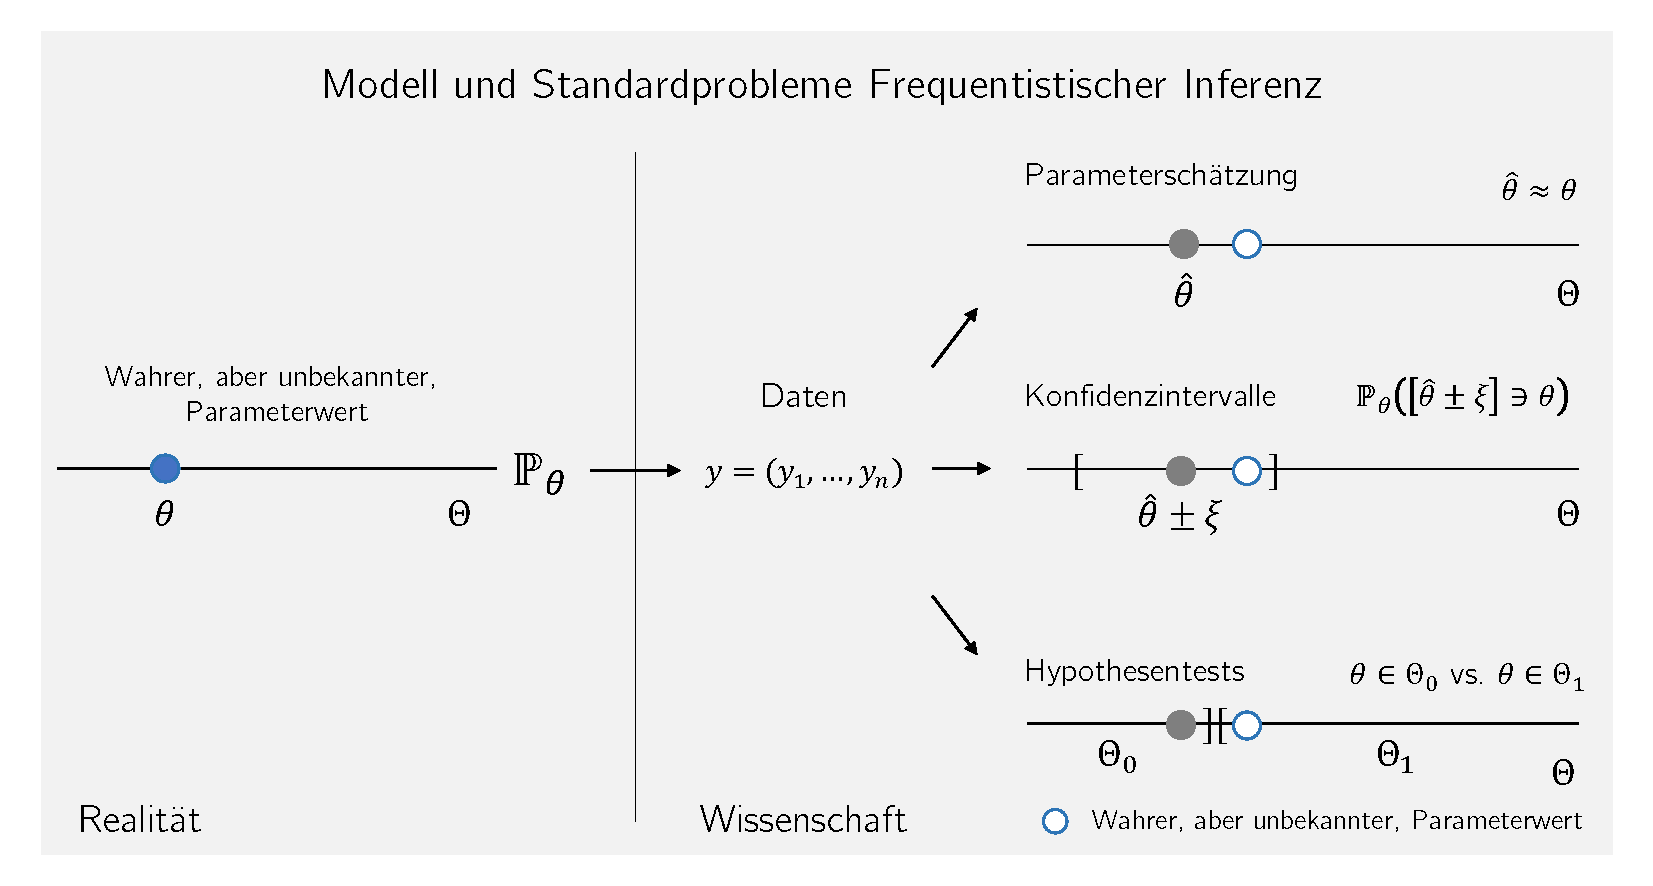
\includegraphics[width=1\linewidth]{9_Abbildungen/wtfi_9_frequentistische_inferenz} \end{center}
\end{frame}

\begin{frame}{Standardprobleme Frequentistischer Inferenz}
\protect\hypertarget{standardprobleme-frequentistischer-inferenz-2}{}
Standardannahmen Frequentistischer Inferenz

\footnotesize

\textbf{\(\mathcal{M}\) sei ein statistisches Modell mit
\(\ups = (\ups_1,...,\ups_n) \sim p_\theta\). Es wird angenommen, dass
ein konkreter Datensatz \(y = (y_1,...,y_n) \in \mathbb{R}^n\) eine der
möglichen Realisierungen von
\(\ups = (\ups_1,...,\ups_n) \sim p_\theta\) ist.}

Aus Frequentistischer Sicht kann man eine Studie unendlich oft
wiederholen und zu jedem Datensatz Schätzer oder Statistiken auswerten,
z.B. das Stichprobenmittel:

\footnotesize
\begin{itemize}
\item[] Datensatz (1) : $y^{(1)} = \left(y_1^{(1)}, y_2^{(1)}, ...,y_n^{(1)}\right)$
                        mit $\bar{y}_n^{(1)} = \frac{1}{n}\sum_{i=1}^n y_i^{(1)}$
\item[] Datensatz (2) : $y^{(2)} = \left(y_1^{(2)}, y_2^{(2)}, ...,y_n^{(2)}\right)$
                        mit $\bar{y}_n^{(2)} = \frac{1}{n}\sum_{i=1}^n y_i^{(2)}$
\item[] Datensatz (3) : $y^{(3)} = \left(y_1^{(3)}, y_2^{(3)}, ...,y_n^{(3)}\right)$
                        mit $\bar{y}_n^{(3)} = \frac{1}{n}\sum_{i=1}^n y_i^{(3)}$
\item[] Datensatz (4) : $y^{(4)} = \left(y_1^{(4)}, y_2^{(4)}, ...,y_n^{(4)}\right)$
                        mit $\bar{y}_n^{(4)} = \frac{1}{n}\sum_{i=1}^n y_i^{(4)}$
\item[] Datensatz (5) : $y^{(5)} = ...$
\end{itemize}

Um die Qualität statistischer Methoden zu beurteilen betrachtet die
Frequentistische Statistik deshalb die Wahrscheinlichkeitsverteilungen
von Schätzern und Statistiken unter Annahme von
\(\ups = (\ups_1,...,\ups_n) \sim p_\theta\). Was zum Beispiel ist die
Verteilung der \(\bar{y}_n^{(1)}\), \(\bar{y}_n^{(2)}\),
\(\bar{y}_n^{(3)}\), \(\bar{y}_n^{(4)}\), \ldots{} also die Verteilung
der Zufallsvariable \(\bar{\ups}_n\)?

Wenn eine statistische Methode im Sinne der Frequentistischen
Standardannahmen ``gut'' ist, dann heißt das also, dass sie bei häufiger
Anwendung ``im Mittel gut'' ist. Im Einzelfall, also im Normalfall nur
eines vorliegenden Datensatzes, kann sie auch ``schlecht'' sein.
\end{frame}

\begin{frame}[t]{Standardprobleme Frequentistischer Inferenz}
\protect\hypertarget{standardprobleme-frequentistischer-inferenz-3}{}
Beispiel \textbar{} Evidenzbasierte Evaluation von Psychotherapie bei
Depression

\begin{center}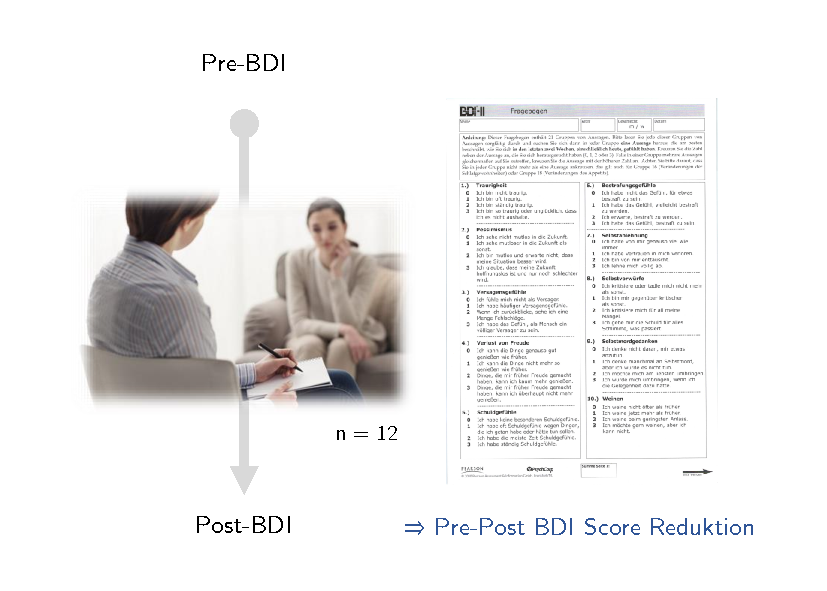
\includegraphics[width=0.9\linewidth]{9_Abbildungen/wtfi_9_messplan} \end{center}
\end{frame}

\begin{frame}[fragile,t]{Standardprobleme Frequentistischer Inferenz}
\protect\hypertarget{standardprobleme-frequentistischer-inferenz-4}{}
Beispiel \textbar{} Evidenzbasierte Evaluation von Psychotherapie bei
Depression

\small
\vspace{2mm}

\footnotesize

\begin{Shaded}
\begin{Highlighting}[]
\NormalTok{fname }\OtherTok{=} \FunctionTok{file.path}\NormalTok{(}\FunctionTok{getwd}\NormalTok{(), }\StringTok{"9\_Grundbegriffe\_Frequentistischer\_Inferenz.csv"}\NormalTok{)}
\NormalTok{D     }\OtherTok{=} \FunctionTok{read.table}\NormalTok{(fname, }\AttributeTok{sep =} \StringTok{","}\NormalTok{, }\AttributeTok{header =}\NormalTok{ T)}
\end{Highlighting}
\end{Shaded}

\vspace{2mm}

\begin{longtable}[]{@{}rr@{}}
\toprule()
i & BDI.Reduktion \\
\midrule()
\endhead
1 & -1 \\
2 & 3 \\
3 & -2 \\
4 & 9 \\
5 & 3 \\
6 & -2 \\
7 & 4 \\
8 & 5 \\
9 & 5 \\
10 & 1 \\
11 & 9 \\
12 & 4 \\
\bottomrule()
\end{longtable}
\end{frame}

\begin{frame}[t]{Standardprobleme Frequentistischer Inferenz}
\protect\hypertarget{standardprobleme-frequentistischer-inferenz-5}{}
Beispiel \textbar{} Evidenzbasierte Evaluation von Psychotherapie bei
Depression \vspace{2mm}

\small

Für die Pre-Post BDI Score Reduktion \(y_i\) der \(i\)ten von \(n\)
Patient:innen legen wir das Modell \begin{equation}
\ups_{i} = \mu + \varepsilon_{i} \mbox{ mit } \varepsilon_{i} \sim N(0,\sigma^2) \mbox{ u.i.v. für } i = 1,...,n
\end{equation} zugrunde. Dabei wird die Pre-Post BDI Reduktion \(y_i\)
der \(i\)ten Patient:in also mithilfe einer über die Gruppe von
Patient:innen identischen Pre-Post BDI Score Reduktion
\(\mu \in \mathbb{R}\) und einer Patient:innen-spezifischen
normalverteilten Pre-Post BDI Score Reduktionsabweichung
\(\varepsilon_{i}\) erklärt

Wie unten gezeigt ist dieses Modell äquivalent zum oben eingeführten
Normalverteilungsmodell \begin{equation}
\ups = (\ups_1,...,\ups_n) \sim N(\mu,\sigma^2).
\end{equation}

Die Standardprobleme der Frequentistischen Inferenz führen in diesem
Szenario auf folgende Fragen:

\begin{enumerate}
[(1)]
\tightlist
\item
  Was sind sinnvolle Tipps für die wahren, aber unbekannten,
  Parameterwerte \(\mu\) und \(\sigma^2\)?
\item
  Wie hoch ist im Frequentistischen Sinn die mit diesen Tipps
  assoziierte Unsicherheit?
\item
  Entscheiden wir uns sinnvollerweise für die Hypothese, dass gilt
  \(\mu\neq 0\) ?
\end{enumerate}
\end{frame}

\begin{frame}[t]{Standardprobleme Frequentistischer Inferenz}
\protect\hypertarget{standardprobleme-frequentistischer-inferenz-6}{}
Beispiel \textbar{} Evidenzbasierte Evaluation von Psychotherapie bei
Depression

\footnotesize

Die Äquivalenz beider Modellformen folgt direkt aus der Transformation
normalverteilter Zufallsvariablen durch linear-affine Funktionen.
Speziell gilt im vorliegenden Fall für
\(\varepsilon_i \sim N(0,\sigma^2)\) u.i.v., dass \begin{equation}
\ups_i = f(\varepsilon_i)
\mbox{ mit }
f : \mathbb{R} \to \mathbb{R}, e_i \mapsto f(e_i) := e_i + \mu.
\end{equation} Dann gilt \begin{align}
\begin{split}
p_{\ups_i}(y_i)
& = \frac{1}{|1|} p_{\varepsilon_i}\left(\frac{y_i - \mu}{1} \right)                        \\
& = N\left(y_i - \mu; 0, \sigma^2\right)                                                    \\
& = \frac{1}{\sqrt{2\pi\sigma^2}}\exp\left(-\frac{1}{2\sigma^2}(y_i - \mu - 0)^2 \right)    \\
& = \frac{1}{\sqrt{2\pi\sigma^2}}\exp\left(-\frac{1}{2\sigma^2}(y_i - \mu)^2 \right)        \\
& = N(y_i; \mu,\sigma^2),
\end{split}
\end{align} also \(\ups_i \sim N(\mu,\sigma^2)\) u.i.v. und damit
\(\ups_1,...,\ups_n \sim N(\mu,\sigma^2)\). \vfill
\end{frame}

\begin{frame}{}
\protect\hypertarget{section-8}{}
\large
\setstretch{3}
\vfill

Statistische Modelle

Statistiken und Schätzer

Standardprobleme Frequentistischer Inferenz

\textbf{Selbstkontrollfragen} \vfill
\end{frame}

\begin{frame}{Selbstkontrollfragen}
\protect\hypertarget{selbstkontrollfragen}{}
\small
\setstretch{2.6}

\begin{enumerate}
\tightlist
\item
  Definieren und erläutern Sie den Begriff des parametrischen
  statistischen Modells.
\item
  Definieren und erläutern Sie den Begriff eine parametrischen
  statistischen Produktmodells.
\item
  Erläutern Sie den Unterschied zwischen univariaten und multivariaten
  statistischen Modellen.
\item
  Formulieren und erläutern Sie das Normalverteilungsmodell.
\item
  Formulieren und erläutern Sie das Bernoullimodell.
\item
  Definieren und erläutern Sie den Begriff der Statistik.
\item
  Definieren und erläutern Sie den Begriff des Schätzers.
\item
  Nennen und erläutern Sie die Standardprobleme der Frequentistischen
  Inferenz.
\item
  Erläutern Sie die Standardannahmen der Frequentistischen Inferenz.
\end{enumerate}
\end{frame}

\end{document}
